\section{Предмет синтаксиса}

\subsection{Синтаксис и другие языковые уровни}
\frame{\tableofcontents[currentsection,currentsubsection]}

\begin{frame}
  \frametitle{Общее определение}

  \begin{block}{Синтаксис}
    \begin{enumerate}
      \item характерные для конкретных языков средства и правила создания речевых единиц;
      \item раздел грамматики, изучающий процессы порождения речи: \begin{itemize}
        \item сочетаемость и порядок следования слов внутри предложения,
        \item а также общие свойства предложения как автономной единицы языка и~высказывания как части текста.
      \end{itemize}
    \end{enumerate}
    [< др.-греч. σύνταξις `построение', `порядок']
  \end{block}
\end{frame}

\begin{frame}
  \frametitle{Уровневая модель языка}

  \begin{table}[t]
    \begin{tabularx}{.9\textwidth}{XXX}
      Уровень & Эмическая единица & Этическая единица \\ \midrule \midrule
      Синтаксис & Предложение & Высказывание \\ \midrule
      \ldots & \ldots & \ldots \\
    \end{tabularx}
  \end{table}

  \onslide<2->{
    \begin{table}[t]
      \begin{tabularx}{.9\textwidth}{XX}
        Уровень & Процесс \\ \midrule \midrule
        Дискурс & Предложение $\rightarrow$ Текст \\ \midrule
        Синтаксис & Слово $\rightarrow$ Предложение \\ \midrule
        Морфология & Морфема $\rightarrow$ Слово \\ \midrule
        Фонология & Фонема $\rightarrow$ Комбинация фонем \\
      \end{tabularx}
    \end{table}
  }
\end{frame}

\begin{frame}
  \frametitle{Модель с центральным положением синтаксиса}
  \framesubtitle{<<Перевернутая Y-модель>>}

  \begin{center}
    \begin{forest}
      [\textit{лексикон} \\ Синтаксис, align=center
        [\textit{синтаксическая структура}
          [Фонологический модуль
            [\textit{фонетическая репрезентация} (PF)]
          ]
          [Семантический модуль
            [\textit{семантическая репрезентация} (LF)]
          ]
        ]
      ]
    \end{forest}
  \end{center}
\end{frame}

\begin{frame}
  \frametitle{Синтаксис и просодика}

  \begin{block}{Интонационные конструкции (Е.\,А.~Брызгунова)}
    \begin{enumerate}
      \item Такие у них обычаи.
      \item \alert{Какие} у них обычаи?
      \item Какие у них \alert{обычаи}?
      \item А у них? Какие у них обычаи?
      \item Какие у них обычаи!
      \item Какие у них \alert{обычаи}!
      \item \alert{Какие} у них обычаи!
    \end{enumerate}
  \end{block}

  \begin{block}<2->{Открытые вопросы}
    \begin{itemize}
      \item Зависимость порядка слов от синтаксической структуры
      \item Взаимозаменяемость синт.\ и прос.\ средств: ср.\ интонация vs клефт
    \end{itemize}
  \end{block}
\end{frame}

\begin{frame}
  \frametitle{Синтаксис и морфология}

  \begin{itemize}
    \item Морфологические формы~--- <<кирпичики>> синтаксических структур
    \item Синтаксические типы словосочетаний во многом дублируют части речи
  \end{itemize}

  \vfill

  \begin{block}{Грамматическая синонимия}
    \begin{itemize}
      \item Компаратив аналитический \textit{(более старый)} vs синтетический \textit{(старше)}
      \item Аналитическое будущее (\textit{буду писать}) vs перфективация \textit{(напишу)}
    \end{itemize}
  \end{block}
\end{frame}

\begin{frame}
  \frametitle{Синтаксис и лексика}

  \begin{itemize}
    \item Лексическое значение накладывает ограничения на синтаксические структуры: неодуш.\ сущ.\ маловероятны как подлежащие при перех.\ гл.
    \item В зависимости от лексического значения различаются синтаксические категории и реализации синтаксических моделей \begin{itemize}
      \item \textit{des vins de France} `происхождение'
      \item \textit{une table de bois} `материал'
      \item \textit{la beauté du paysage} `качество'
    \end{itemize}
    \item Синтаксическая структура дифференцирует значения слова: ср.\ \textit{décoller qch} vs \textit{l'avion a décollé}
  \end{itemize}
\end{frame}

\begin{frame}
  \frametitle{Параллельная модель (Р.~Джекендофф)}
  \small

  \begin{columns}
    \column{.33\textwidth}
    \begin{forest}
      [Фонология \\ (фонологические правила), align=center
        [\subnode{ph}{\textit{фонологические структуры}}, align=center]
      ]
    \end{forest}
    \column{.33\textwidth}
    \begin{forest}
      [Синтаксис \\ (синтаксические правила), align=center
        [\subnode{sx}{\textit{синтаксические структуры}}, align=center]
      ]
    \end{forest}
        \column{.33\textwidth}
    \begin{forest}
      [Семантика \\ (семантические правила), align=center
        [\subnode{sm}{\textit{концептуальные структуры}}, align=center]
      ]
    \end{forest}
  \end{columns}

  \begin{tikzpicture}[overlay,remember picture,<->,black,dashed,bend angle=45,bend right]
    \draw($(pic cs:ph)+(1,-1.6)$) to ($(pic cs:sx)+(-1,-1.6)$);
    \draw($(pic cs:sx)+(1,-1.6)$) to ($(pic cs:sm)+(-1,-1.6)$);
    \draw ($(pic cs:ph)+(0,-1.6)$) to ($(pic cs:sm)+(0,-1.6)$);
  \end{tikzpicture}
\end{frame}

\subsection{Подходы к описанию синтаксиса}
\frame{\tableofcontents[currentsection,currentsubsection]}

\begin{frame}
  \frametitle{Треугольник Фреге}
  \centering

  \begin{tikzpicture}
    \draw (0,0) node[anchor=south]{Знак}
    -- (2,-4) node[anchor=north]{Смысл}
    -- (-2,-4) node[anchor=north]{Значение}
    -- cycle;
  \end{tikzpicture}
\end{frame}

\begin{frame}
  \frametitle{Основные подходы}

  \begin{enumerate}
    \item \textbf{Структурный:} языковые формы рассматриваются в самом себе безотносительно к отображаемой ими действительности ($\sim$ знак)
    \item \textbf{Логический:} языковая форма сопоставляется со структурой логического суждения ($\sim$ значение)
    \item \textbf{Семантический:} сопоставление со структурой действительности, описываемой при помощи формы ($\sim$ смысл)
  \end{enumerate}
\end{frame}

\begin{frame}
  \frametitle{Коммуникативный синтаксис}

  \begin{itemize}
    \item Актуальное членение (< Ш.~Балли: thème и propos)
    \item Порядок слов
    \item Коммуникативная парадигматика: \begin{itemize}
      \item Она кричала \textit{громко}. $\downarrow$~--- рема
      \item Она \textit{громко} кричала. $\downarrow$~--- рематический модификатор
      \item \textit{Громко} $\uparrow$ | она не кричала. $\downarrow$~--- контрастная тема
    \end{itemize}
  \end{itemize}
\end{frame}

\begin{frame}
  \frametitle{Прагматический синтаксис}

  \begin{block}{Прагматика по Моррису}
    Раздел семиотики, изучающий отношение знака к субъекту
  \end{block}

  \vfill

  Типы речевых актов и выражающих их синтаксических структур:
  \begin{itemize}
    \item Констатив $\sim$ повествовательное предложение
    \item Реквестив $\sim$ вопросительное \textit{или} повествовательное
    \item \ldots
  \end{itemize}
\end{frame}

\begin{frame}
  \frametitle{Трансформационный синтаксис}

  \begin{itemize}
    \item Синтаксис делится на ядерную (исходную) подсистему и производную
    \item Тип ядерных предложений описывает класс элементарных ситуаций
    \item Сложный тип = ядерные предложения + набор правил преобразования
  \end{itemize}
\end{frame}

\begin{frame}
  \frametitle{Виды трансформаций}

  \begin{enumerate}
    \item \textbf{Количественные:} добавление или опущение элемента
    \item \textbf{Качественные:} замена элемента
    \item \textbf{Перестановочные:} изменение расположения элементов
  \end{enumerate}

  \vfill

  \begin{block}<2->{Качественные}
    \begin{enumerate}
      \item Изменение морфологической формы: \textit{Demain il part $\rightarrow$ partira pour Paris}
      \item Транспозиция: \textit{Il écoutait attentivement $\rightarrow$ avec attention}
      \item Актантная деривация: \textit{La maison est construite pas les ouvriers}
      \item Трансформация форм связи: \textit{Je n'ai pas vu l'homme dont vous m'avez parlé}
    \end{enumerate}
  \end{block}
\end{frame}

\section{Синтаксические объекты}

\subsection{Предложение}
\frame{\tableofcontents[currentsection,currentsubsection]}

\begin{frame}
  \frametitle{Текст}

  Свойства: \begin{enumerate}
    \item Законченность (оценка со стороны говорящего)
    \item Целостность (со стороны слушающего)
  \end{enumerate}

  \vfill

  $\rightarrow$ Сверхфразовое единство \\
  $\rightarrow$ Простое предложение \\
  $\rightarrow$ Словосочетание \\
  $\rightarrow$ Слово
\end{frame}

\begin{frame}
  \frametitle{Особенности синтаксических объектов}

  \begin{itemize}
    \item (Счетная) бесконечность множества
    \item Способность к неограниченному усложнению \begin{itemize}
      \item Добавление зависимого слова к одному из компонентов
      \item Подчинение всего выражения новой синтаксической вершине
    \end{itemize}
  \end{itemize}
\end{frame}

\begin{frame}
  \frametitle{Предложение}

  Синтаксическая конструкция, которая является \begin{itemize}
    \item относительно независимым от контекста высказыванием,
    \item обладающим коммуникативной функцией
    \item и интонационным оформлением,
    \item включающим грамматически связанные формы слов
    \item и построенным на основе отвлеченного грамматического образца~--- структурной схемы.
  \end{itemize}
\end{frame}

\begin{frame}
  \frametitle{Предикативность}

  \begin{block}{Предикация}
    Установление связи между предложением и ситуацией
  \end{block}

  \vfill

  \begin{itemize}
    \item \textit{Лошадь белая}~--- связь устанавливается в самом предложении
    \item \textit{Белая лошадь}~--- есть пресуппозиция, что связь уже существует
  \end{itemize}
\end{frame}

\subsection{Словосочетание}
\frame{\tableofcontents[currentsection,currentsubsection]}

\begin{frame}
  \frametitle{Словосочетание}

  Синтаксическая конструкция, образующаяся на основе подчинительных связей. Обязательно есть главный компонент (вершина) и 1+ зависимых

  \vfill

  \begin{block}<2->{Критерии}
    \begin{enumerate}
      \item Грамматический~--- отсутствие предикативности
      \item Функциональный~--- расчлененное выражение понятия
      \item Структурный~--- конструкция из 2+ словоформ, связанных СинтО
      \item Семантический~--- выражение СинтО
      \item Парадигматический~--- система форм, изоморфная парадигме вершины
    \end{enumerate}
  \end{block}

\end{frame}

\begin{frame}
  \frametitle{Классификация}

  \begin{itemize}
    \item По частеречной принадлежности вершины \begin{itemize}
      \item Глагольные
      \item Субстантивные
      \item Адъективные
      \item Наречные
    \end{itemize}
    \item Свободные vs несвободные~--- по наличию комплетивной связи
    \item По типу конструктивной сложности \begin{itemize}
      \item Простое: \textit{верблюжья шерсть}
      \item Сложное (куст): \textit{гладкая верблюжья шерсть}
      \item Комбинированное (дерево): \textit{пальто из верблюжьей шерсти}
    \end{itemize}
  \end{itemize}
\end{frame}

\section{Представление синтаксической структуры}
\frame{\tableofcontents[currentsection]}

\begin{frame}
  \frametitle{Отношения вложения}

  \Tree [.S [.NP This ] [.VP [.V is ] [.NP an example sentence. ] ] ]
\end{frame}

\begin{frame}
  \frametitle{Отношения подчинения}

  \begin{center}

    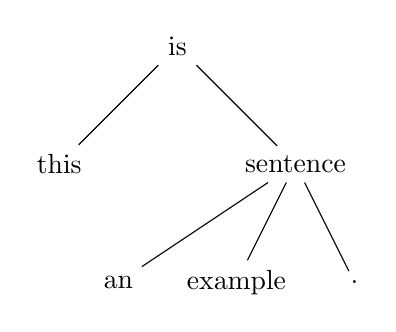
\begin{tikzpicture}
      \node (is-root) {is}
      [sibling distance=3cm]
      child { node {this} }
      child {
        node {sentence}
        [sibling distance=1.5cm]
        child { node {an} }
        child { node {example} }
        child { node {.} }
        child[missing]
      };
    \end{tikzpicture}
  \end{center}
\end{frame}
